\documentclass[12pt]{article}

\usepackage[german]{babel}
\usepackage{amsmath}
\usepackage{amssymb} % to display symbols for real numbers, integers etc. Usage: \mathbb{R}
\usepackage{graphicx}
\usepackage{listings} % to display programming code
%\usepackage[ngerman]{babel}
\usepackage{color}
\usepackage{relsize} % to display scaled math symbols (big summation symbol etc.)
\usepackage{textcomp}

\DeclareGraphicsExtensions{.pdf,.jpeg,.png}
\definecolor{listinggray}{gray}{0.9}
\definecolor{lbcolor}{rgb}{0.9,0.9,0.9}
\lstset{ % to display programming code in nice colors
	backgroundcolor=\color{lbcolor},
	tabsize=4,
	rulecolor=,
	language=matlab,
		basicstyle=\scriptsize, %for extra small font size
        upquote=true,
        aboveskip={1.5\baselineskip},
        columns=fixed,
        showstringspaces=false,
        extendedchars=true,
        breaklines=true,
        prebreak = \raisebox{0ex}[0ex][0ex]{\ensuremath{\hookleftarrow}},
		frame=single, %draw frame
        showtabs=false,
        showspaces=false,
        showstringspaces=false,
        identifierstyle=\ttfamily,
        keywordstyle=\color[rgb]{0,0,1},
        commentstyle=\color[rgb]{0.133,0.545,0.133},
        stringstyle=\color[rgb]{0.627,0.126,0.941},
        numbers=left,
        stepnumber=1,
        firstnumber=1,
        numberfirstline=true,
        linewidth=14cm,
}

\title{\"Ubungsblatt 7\\ \glqq Mustererkennung\grqq}
\author{J. Cavojska, N. Lehmann, R. Toudic}
\date{16.06.2015}
\begin{document}
\maketitle
%\renewcommand{\contentsname}{Table of Contents}
\tableofcontents
\newpage

\section{Logistische Regression}

\subsection{Code}

\begin{lstlisting}[language=Matlab]
% Clean up
clear all
close all
clc

% Datenaufbereitung
Data         = load('fieldgoal.txt');
ExtendedData = [Data(:,1), ones(size(Data,1), 1)];
Distance     = Data(:,1);
Goal         = Data(:,2);
x01          = linspace(0,1);
x0100        = linspace(0,100);
N            = length(Data);
limit        = 100000;
plist        = [];

%%% Aufgabe 1 - Logistische Regression %%%

alpha = 10^(-7);
beta  = [0,0];   % initiales beta

for repeats = 1:limit
    
    likelihood = 0;
    e          = 0;
    
    for i = 1:N
    
        k = beta*ExtendedData(i,:)';
        p = exp(k)/(1+exp(k));
        likelihood = likelihood + Distance(i) * ( Goal(i) - p );
        e = e + abs(Goal(i) - p);

    end

    beta = beta + (alpha * likelihood);
    plist = vertcat(plist,p);
    
    if mod(repeats,25000) == 0
        e
    end
end

% Diskriminante
fx = beta(1) * beta(2)*x0100;

% plot
figure('NumberTitle','off','Name','Aufgabe 1 - Logistische Regression');
hold on
  
scatter(Distance, Goal);
plot(plist, 'g');
plot(fx);

title('Aufgabe 1 - Logistische Regression');
xlabel('Distanz zum Tor');
ylabel('Wahrscheinlichkeit für einen Treffer')
axis([-0.1 100.1 -0.1 1.1]);
legend('Datenpunkte','p(x,beta)','Diskriminante');

% error-output
% 351.1322
% 351.1322
% 351.1322
% 351.1322
\end{lstlisting}

\subsection{Bilder}

\begin{center}
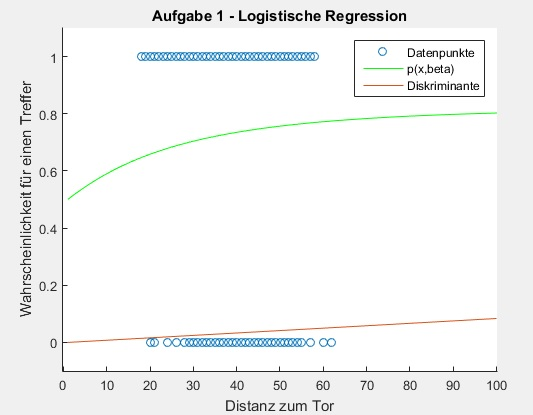
\includegraphics[width=10cm]{plot.jpg}
\end{center}


\end{document}